\documentclass{beamer}
\usepackage{up}

\title{Побитови операции}

\date{23 ноември 2016 г.}

\titlegraphic{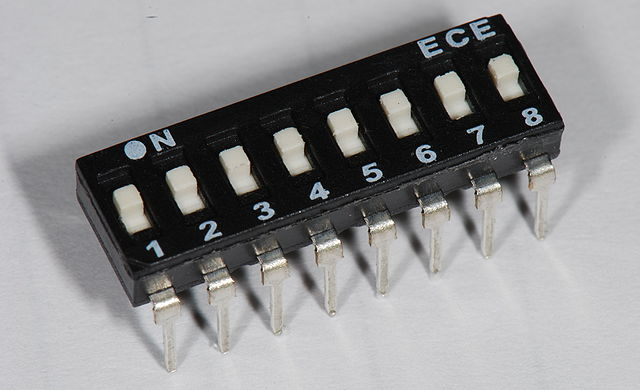
\includegraphics[height=0.3\textheight]{images/dipswitch.jpg}}

\begin{document}

\begin{frame}
  \titlepage
\end{frame}

\section{Побитови операции в C++}

\begin{frame}
  \frametitle{Логически битови операции}

  \begin{center}
    \begin{tabular}{c@{\hskip 12ex}c}
      Конюкнция & Дизюкнция\\[1em]
      \begin{tabular}{c|c|c}
        \tt\&&0&1\\
        \hline
        0&0&0\\
        \hline
        1&0&1\\
      \end{tabular}
      &
        \begin{tabular}{c|c|c}
          \tt|&0&1\\
          \hline
          0&0&1\\
          \hline
          1&1&1\\
        \end{tabular}\\[3em]
      Изключващо или & Отрицание\\[1em]
      \begin{tabular}{c|c|c}
        \tt\^&0&1\\
        \hline
        0&0&1\\
        \hline
        1&1&0\\
      \end{tabular}
      &
        \begin{tabular}{c|c}
          \tt\~&\\
          \hline
          0&1\\
          \hline
          1&0
        \end{tabular}
    \end{tabular}
  \end{center}
\end{frame}

\begin{frame}[<1-2>]
  \frametitle{Побитови операции}

  \begin{center}
    \begin{tabular}{cc}
      \begin{bittable}
        \multirow{2}{*}{\tt\&}
        &0&0&1&0&1&0&1&0\\
        &1&0&1&0&0&0&1&1\\
        \hline
        &0&0&1&0&0&0&1&0
      \end{bittable}
      &
      \begin{bittable}
        \multirow{2}{*}{\tt|}
        &0&0&1&0&1&0&1&0\\
        &1&0&1&0&0&0&1&1\\
        \hline
        &1&0&1&0&1&0&1&1
      \end{bittable}\\[3em]
      \begin{bittable}
        \multirow{2}{*}{\tt\^}
        &0&0&1&0&1&0&1&0\\
        &1&0&1&0&0&0&1&1\\
        \hline
        \onslide<2->{\multirow{2}{*}{\tt\^}}
        &1&0&0&0&1&0&0&1
        \onslide<2->{\\
        &1&0&1&0&0&0&1&1\\
        \hline
        &0&0&1&0&1&0&1&0}
      \end{bittable}
      &
      \begin{bittable}
        \tt\~
        &0&0&1&0&1&0&1&0\\
        \hline
        \onslide<2->{\tt\~}&1&1&0&1&0&1&0&1
        \onslide<2->{\\
        &0&0&1&0&1&0&1&0}      
      \end{bittable}
    \end{tabular}
  \end{center}
\end{frame}

\begin{frame}
  \frametitle{Побитово изместване}
  \begin{center}

    \begin{bittable}
      \tt{>{}>2}&1&0&1&0&1&1&\cellcolor{gray!25}0&\cellcolor{gray!25}1\\
      \hline
      &\cellcolor{yellow}0&\cellcolor{yellow}0&1&0&1&0&1&1
    \end{bittable}
    \vspace{1em}

    \tt{a >{}> x} $\quad\longleftrightarrow\quad$ \tt{a / $2^{\tt x}$}
    \vspace{3em}

    \begin{bittable}
      \tt{<{}<2}&\cellcolor{gray!25}1&\cellcolor{gray!25}0&1&0&1&1&0&1\\
      \hline
      &1&0&1&1&0&1&\cellcolor{yellow}0&\cellcolor{yellow}0
    \end{bittable}
    \vspace{1em}

    \tt{a <{}< x} $\quad\longleftrightarrow\quad$ \tt{a * $2^{\tt x}$ \% $2^8$}
  \end{center}
\end{frame}

\section{Числата като масиви от битове}

\begin{frame}
  \frametitle{Маски}
  \begin{center}
    \begin{tabular}{cc}
      \multicolumn{2}{c}{Записване на битове}\\[1em]
      \begin{bittable}
        \multirow{2}{*}{\tt\&}
        &0&0&1&0&1&\cellcolor{green}1&1&0\\
        &1&1&1&1&1&\cellcolor{red}0&1&1\\
        \hline
        &0&0&1&0&1&\cellcolor{red}0&1&0
      \end{bittable}
      &
      \begin{bittable}
        \multirow{2}{*}{\tt|}
        &0&0&1&\cellcolor{red}0&1&1&1&0\\
        &0&0&0&\cellcolor{green}1&0&0&0&0\\
        \hline
        &0&0&1&\cellcolor{green}1&1&1&1&0
      \end{bittable}\\[3em]
      \multicolumn{2}{c}{Прочитане на битове}\\[1em]
      \begin{bittable}
        \multirow{2}{*}{\tt\&}
        &0&0&1&0&1&\cellcolor{green}1&1&0\\
        &0&0&0&0&0&\cellcolor{yellow}1&0&0\\
        \hline
        &0&0&0&0&0&\cellcolor{green}1&0&0
      \end{bittable}
      &
      \begin{bittable}
        \multirow{2}{*}{\tt\&}
        &0&0&1&\cellcolor{red}0&1&1&1&0\\
        &0&0&0&\cellcolor{yellow}1&0&0&0&0\\
        \hline
        &0&0&0&\cellcolor{red}0&0&0&0&0
      \end{bittable}\\[3em]
    \end{tabular}
  \end{center}
\end{frame}

\begin{frame}[<1-3>]
  \frametitle{Операции с маски}
  \begin{center}
    \begin{tabular}{cc}
      \multicolumn{2}{c}{Конструиране на маски}\\[1em]
      \begin{bittable}
        \tt{<{}<3}
        &0&0&0&0&0&0&0&\cellcolor{green}1\\
        \hline
        \onslide<2->{\tt\~}&0&0&0&0&\cellcolor{green}1&0&0&0
        \onslide<2->{\\
          \hline
          &1&1&1&1&\cellcolor{red}0&1&1&1\\
        }
      \end{bittable}
      &
      \begin{bittable}
        \tt{<{}<3}
        &0&0&0&0&0&0&0&\cellcolor{green}1\\
        \hline
        -1&0&0&0&0&\cellcolor{green}1&0&0&0\\
        \hline
        \onslide<2->{\tt\~}&0&0&0&0&0&\cellcolor{green}1&\cellcolor{green}1&\cellcolor{green}1
        \onslide<2->{\\
          \hline
          &1&1&1&1&1&\cellcolor{red}0&\cellcolor{red}0&\cellcolor{red}0
        }
      \end{bittable}\onslide<3->{\\[3em]
      \multicolumn{2}{c}{Комбиниране на маски}\\[1em]
      \begin{bittable}
        \multirow{2}{*}{\tt|}
        &0&0&0&0&\cellcolor{green}1&0&0&0\\
        &0&0&\cellcolor{green}1&0&0&0&0&0\\
        \hline
        &0&0&\cellcolor{green}1&0&\cellcolor{green}1&0&0&0\\
      \end{bittable}
      &
      \begin{bittable}
        \multirow{2}{*}{\tt\&}
        &1&1&\cellcolor{red}0&1&1&1&1&1\\
        &1&1&1&1&1&\cellcolor{red}0&1&1\\
        \hline
        &1&1&\cellcolor{red}0&1&1&\cellcolor{red}0&1&1\\
      \end{bittable}
      }
    \end{tabular}
  \end{center}
\end{frame}

\end{document}
